\documentclass[12pt]{article}
\usepackage[utf8]{inputenc}
\usepackage{wrapfig}
\usepackage{Preambles/preamble}

\newcommand{\mycomment}[1]{}

%~~~~~~~~~~~~~~~~~~~~~~~~~~~~~~~~~~~~~~~~~~~~~~~~~~~~~~~~~~~~~~~~~~~~~~~~~~~~~~~~~~~~~~~~~~~~~~%
%%%%%%%%%%%%%%%%%%%%%%%%%%%%%%%%%%%%%%%%%%%%%%%%%%%%%%%%%%%%%%%%%%%%%%%%%%%%%%%%%%%%%%%%%%%%%%%%
%                                                                                              % 
%             Template produced by Fergus Babb of the University of Nottingham, 2024           %
%                                                                                              %  
%%%%%%%%%%%%%%%%%%%%%%%%%%%%%%%%%%%%%%%%%%%%%%%%%%%%%%%%%%%%%%%%%%%%%%%%%%%%%%%%%%%%%%%%%%%%%%%%
%~~~~~~~~~~~~~~~~~~~~~~~~~~~~~~~~~~~~~~~~~~~~~~~~~~~~~~~~~~~~~~~~~~~~~~~~~~~~~~~~~~~~~~~~~~~~~~%

\begin{document}

%%%%%%%%%%%%%%%%%%%%%%%%%%%%%%%%%%%%%%%%%%%%%%%%%%%%%%%%%%%%%%%%%%%%%%%%%%%%%%%%%%%%%%%%%%%%%%%%
\title{Management of security : GASEO -  Global Agency for Satellite Earth Observation}
%This isn't supposed to be for level of authorship, alphabetical is fine
\firstauthor{Alexandre Vinovrski}
\firstID{000501157}
\firstemail{vinovrski.alexandre@ulb.be}
\submitdate{\today}
\maketitle

\addtocounter{page}{-1}
\pagenumbering{roman}
\thispagestyle{empty}
%%%%%%%%%%%%%%%%%%%%%%%%%%%%%%%%%%%%%%%%%%%%%%%%%%%%%%%%%%%%%%%%%%%%%%%%%%%%%%%%%%%%%%%%%%%%%%%%

%\newpage
%\null\vspace{2in}
%\begin{abstract}
%\blindtext 
%\end{abstract}
%\vspace{\fill}
%\thispagestyle{empty}

%~~~~~~~~~~~~~~~~~~~~~~~~~~~~~~~~~~~~~~~~~~~~~~~~~~~~~~~~~~~~~~~~~~~~~~~~~~~~~~~~~~~~~~~~~~~~~~~

\newpage
\doublespacing
\tableofcontents
\singlespacing

%~~~~~~~~~~~~~~~~~~~~~~~~~~~~~~~~~~~~~~~~~~~~~~~~~~~~~~~~~~~~~~~~~~~~~~~~~~~~~~~~~~~~~~~~~~~~~~~
%Sections before Main Content of report

%\newpage
%\section*{Conventions and Notation}\label{Conventions}
%\addcontentsline{toc}{subsection}{\textit{Conventions and Notation}}
%\begin{enumerate}[i.]
%\item A convention you use here, e.g. Unless otherwise stated we use units such that $c=1$.
%\end{enumerate}

%\vspace{2em}

%\addcontentsline{toc}{subsection}{\textit{Acronyms}}
%\printacronyms
%\newacronym{acrlabel}{ABC}{Definition}
%\vspace{2em}

%\listoffigures
%\addcontentsline{toc}{subsection}{\textit{List of Figures}}
%\vspace{2em}

%\listoftables
%\addcontentsline{toc}{subsection}{\textit{List of Tables}}
%\vspace{2em}
%\newpage

%\section*{Acknowledgements}\label{Acknowledgements}
%\addcontentsline{toc}{subsection}{\textit{Acknowledgements}}
%\vspace{2em}

%\section*{Preface}\label{Preface}
%\addcontentsline{toc}{subsection}{\textit{Preface}}
%\vspace{2em}
%\blindtext

%~~~~~~~~~~~~~~~~~~~~~~~~~~~~~~~~~~~~~~~~~~~~~~~~~~~~~~~~~~~~~~~~~~~~~~~~~~~~~~~~~~~~~~~~~~~~~~~
%Main Content sections start

\newpage
\pagenumbering{arabic}
%\section*{Main Content}%So pdf viewers dont have everything as a subsection of preamble
\addcontentsline{toc}{part}{Main content}


\section{Context} \label{Sec: Context}



\subsection{GASEO description}
The Global Agency for Satellite Earth Observation (GASEO) collaborates with both the general public and governmental entities, offering a spectrum of satellite image services tailored to various needs.

\subsection{GASEO for Public Access}
GASEO offers the general public access to satellite images at lower resolutions, allowing them to purchase specific images for search and download purposes.
Sensitive areas such as military bases are not accessible to the public, related images are blurred and not downloadable. 
Customers have the option to either pay per image to download or subscribe to various plans.
These subscription plans offer different tiers, with higher-tier subscriptions providing access to a greater number of downloadable images. 
Customers have the option to conduct restricted searches for free without requiring an account. In this case images are not downloadable.

\subsection{GASEO for Governmental Agencies}
Authorized governmental agencies benefit from higher resolution satellite images, enabling them to conduct detailed searches and downloads. Additionally, these agencies can subscribe to designated regions for which GASEO provides specialized reports and updates.

\subsection{GASEO Registration process}
The website and web interface used by governmental agencies differ from those utilized by the general public for typical actions. 

The registration process for the general public is straightforward, involving account creation, password registration, and setting up double authentication for added security.

Given GASEO's headquarters in Belgium, not all agencies can register and access its interface. 
Governmental agencies from countries outside the European Union are not granted access to GASEO tools if they do not comply with EU regulations. 

\newpage
%~~~~~~~~~~~~~~~~~~~~~~~~~~~~~~~~~~~~~~~~~~~~~~~~~~~~~~~~~~~~~~~~~~~~~~~~~~~~~~~~~~~~~~~~~~~~~~~

\section{Business Processes}\label{Sec: Processes}

\subsection{GASEO Public Website Diagrams}
\subsubsection*{Use Case}

\begin{figure}[h]
    \centering
    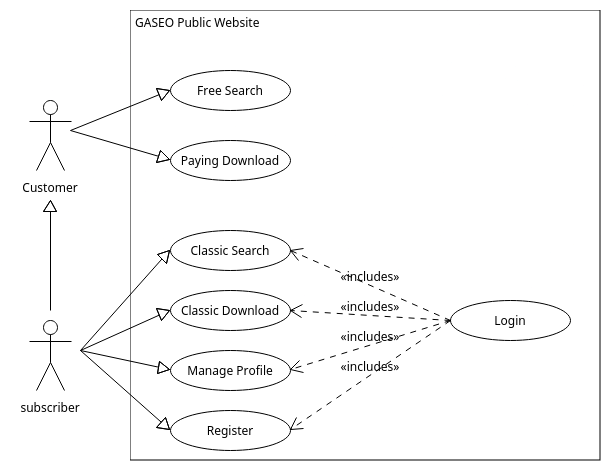
\includegraphics[width=0.35\textwidth]{Figures/Business Processes/UseCase_1.png}
    \caption{User and Subscriber use case diagram}
\end{figure}

\begin{itemize}
  \item \textbf{Customer} can search freely on the GASEO public website and pay to download specific image.
  \item \textbf{Subscriber} inherit from \textbf{Customer} and can perform classic search, classic download, manage his profile, and register to a specific subscription plan.
\end{itemize}


\subsubsection*{Activity Diagrams}

\begin{figure}[h]
    \centering
    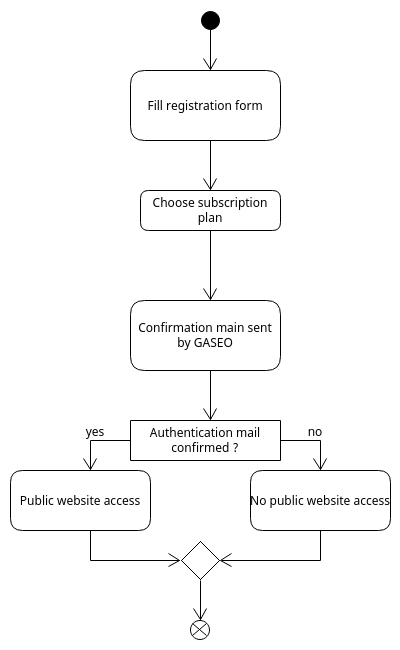
\includegraphics[width=0.25\textwidth]{Figures/Business Processes/Activity_1.png}
    \caption{Customer Registration process.}
\end{figure}

\begin{itemize}
    \item A registration form is given to the customer asking him his basic credentials like mail, password, phone number for double authentication and motivation (Business purpose, school purpose, etc.)
    \item The customer choose it's subscription plan, and give his bank account information.
    \item Confirmation mail is sent to the customer via it's given mail address. The customer has 24 hours to validate its mail.
\end{itemize}

\begin{figure}[h]
    \centering
    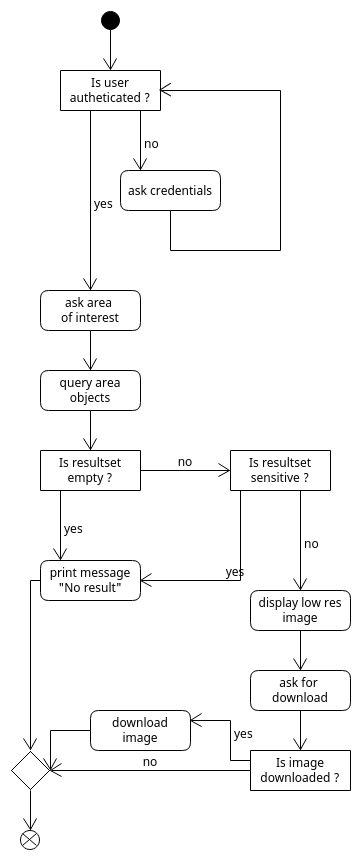
\includegraphics[width=0.25\textwidth]{Figures/Business Processes/Activity_2.png}
    \caption{Customer data search.}
\end{figure}

\begin{itemize}
    \item User is asked it's credential to connect to GASEO public website. Connection is authorised after double identification by phone number.
    \item After login, user is asked to search for area of interest. Based on the type of area, the search engine might limits the result set. Finally, the user is able to download images from result set.
\end{itemize}

\newpage

\begin{figure}[h]
    \centering
    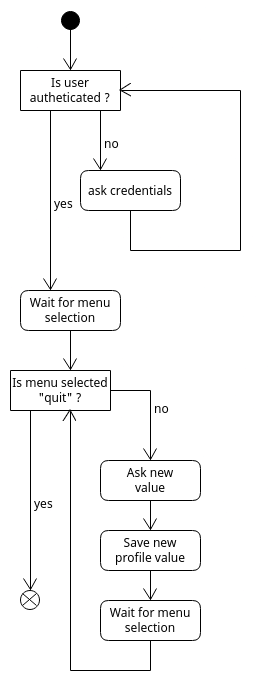
\includegraphics[width=0.25\textwidth]{Figures/Business Processes/Activity_3.png}
    \caption{ Customer profile management.}
\end{figure}

\begin{itemize}
    \item User is asked it's credential to connect to GASEO public website. Connection is authorised after double identification by phone number.
    \item Once identified, user has the abilities to change default credential like mail, phone number, password etc. Note that if the mail or the phone number is changed, a confirmation mail or SMS will be sent. If confirmation is not established, the value will fall back to the previous one.
\end{itemize}

\newpage
\subsection{GASEO Private Website Diagrams}
\subsubsection*{Use Case}
\begin{figure}[h]
    \centering
    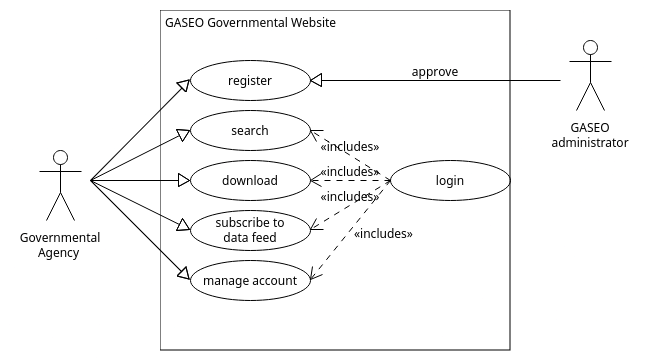
\includegraphics[width=0.5\textwidth]{Figures/Business Processes/UseCase_2.png}
    \caption{Agency use case diagram.}
\end{figure}

\begin{itemize}
  \item \textbf{Governmental agencies} can introduce a demand to register on the GASEO's official portal available on their website. Registration requires sending an email from a recognized official email address along with a justification for registration. Verification of the agency's recognition is essential before registration is approved.
  \item  \textbf{A GASEO administrator} validate or not the demand, and register manually the user if the the demand is accepted. It's important to note that only an administrator can register an agency. Once the account has been created, a one time use password is sent by mail after being encrypted with a symmetric cryptography system.
  \item After demand approval, governmental agencies get encrypted password, login, change password and gain access to comprehensive features on the GASEO portal. This includes the ability to conduct full searches, download high-resolution images, subscribe to regional areas, and manage their accounts.
\end{itemize}

\newpage
\subsubsection*{Activity Diagram}
\begin{figure}[h]
    \centering
    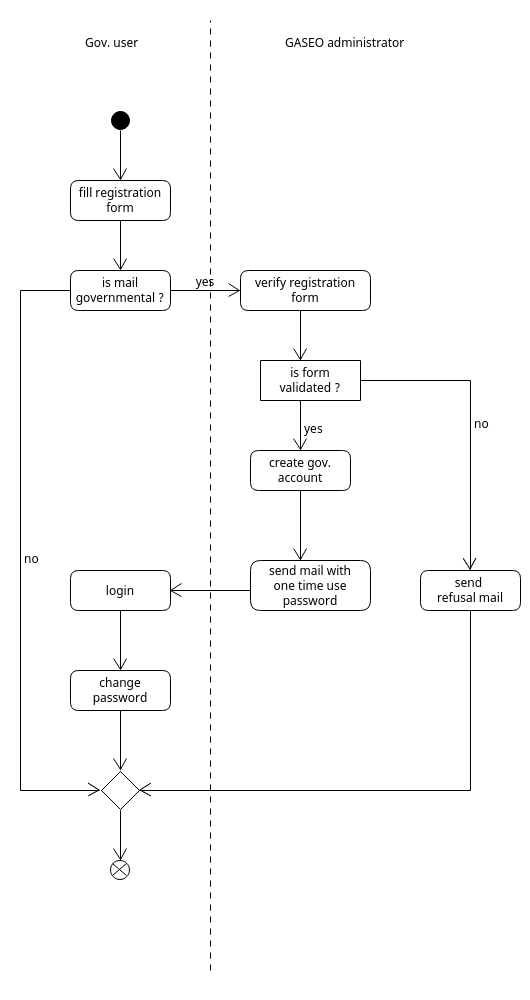
\includegraphics[height=0.65\textwidth]{Figures/Business Processes/Activity_4.png}
    \caption{Governmental User registration process.}
\end{figure}

Governmental Customer data search and profile management are basically the same as classical customer. 

As described in section \ref{Sec: Context} the registration process is done by a GASEO administrator after the governmental agency has filled the registration form.

\newpage
\subsubsection*{Data Flow Diagram}
\begin{figure}[h]
    \centering
    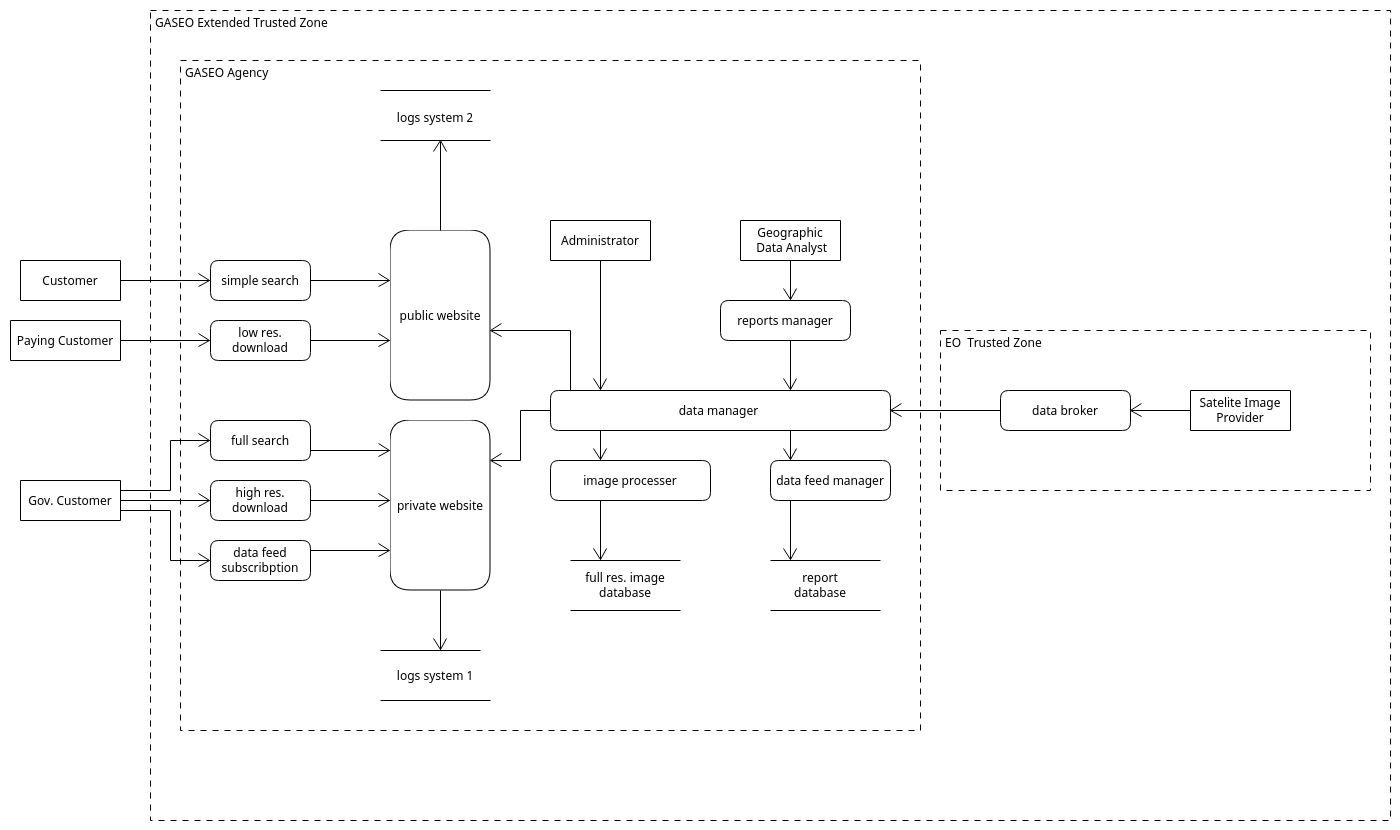
\includegraphics[width=\textwidth]{Figures/Business Processes/DataFlow_1.png}
    \caption{Data Flow Diagram for GASEO.}
\end{figure}

It's crucial to emphasize the distinction between a public website and a private one in cases of intrusion. This demarcation is essential because public users should not have access to sensitive information. Hence, it's imperative to thwart any attempts by public users to discover government agent passwords and accounts, necessitating the separation.

\newpage

%~~~~~~~~~~~~~~~~~~~~~~~~~~~~~~~~~~~~~~~~~~~~~~~~~~~~~~~~~~~~~~~~~~~~~~~~~~~~~~~~~~~~~~~~~~~~~~~
\section{Infrastructure Situation}\label{Sec: Infrastructure}

Here's the current GASEO network topology : 


\begin{figure}[h]
    \centering
    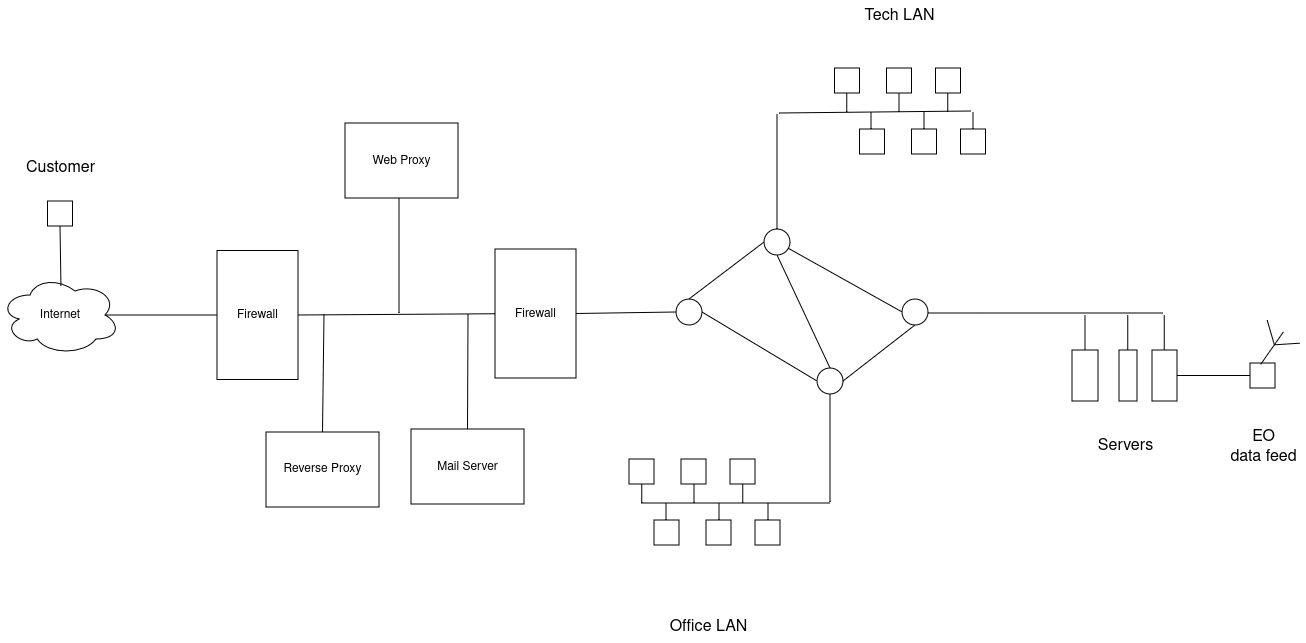
\includegraphics[width=0.9\textwidth]{Figures/Infrastructure/Topology_1.png}
    \caption{Network Topology - A second web server can be added to correspond to DFD at figure 5.}
\end{figure}

This network is relatively flat and might lead to security and performance issues : 
\begin{itemize}
    \item The\textbf{ Firewalls }divide the network into three segments: Internet, Service/DMZ, and Internal. Double firewall prevent single point of failure however this division may not offer adequate protection for the internal network as LANs and servers reside within the same trusted zone creating a relatively flat structure.
    
    The firewall on the Internet side must be configured to handle incoming spoofed packets from the Internet containing internal IP addresses.
    
    The internal-side firewall should only allow incoming packets from IP addresses within the designated range for the Service zones.
    
    \item The \textbf{Reverse Proxy} and \textbf{Web Proxy} are responsible for managing incoming requests and prevent the exposure of the entire network topology. They also assist in policy enforcement and traffic inspection.
    
    \item Separation is made between \textbf{Office LAN} and \textbf{Tech LAN} to prevents single point of failure ,limits the potential impact of a security breach on one LAN to the other LAN.
    
    \item The absence of an Intrusion Detection System (\textbf{IDS}) on the internal side of the network may result in insufficient network inspection.

    \item Finally, \textbf{Servers} are in the internal zone of the network. Servers are tasked with  managing active directory, email, data feeds from \textbf{EO}, and providing access to databases.
\end{itemize}
\newpage
%~~~~~~~~~~~~~~~~~~~~~~~~~~~~~~~~~~~~~~~~~~~~~~~~~~~~~~~~~~~~~~~~~~~~~~~~~~~~~~~~~~~~~~~~~~~~~~~
\section{Risk Assessment}\label{Sec: Assessment}

\subsection{Threats}
Based on the \textbf{STRIDE} model, we will discuss potential threats possible on our system with a non exhaustive list.

\subsubsection*{Spoofing}
\begin{itemize}
    \item \textbf{ T1 Customer Spoofing}: A traditional non-paying customer has the ability to pose as a paying subscriber or a government client. While the former scenario may seem less severe as low-resolution images contain less sensitive data, it could also be more challenging identifying. In contrast, spoofing as a government entity in the second case could lead to more significant information leakage and information disclosure.
    
    \item \textbf{ T2 IP Spoofing }: An attacker on the internet side may send a packet with spoofed internal network IP addresses, allowing it to bypass the firewall. Sending such spoofed packets to an internal workstation could potentially compel it to reconnect to external networks.

    \item \textbf{ T3 Protocol Based Spoofing }: Depending on if the malicious actors is inside the GASEO network or outside, ARP DHCP or DNS spoofing might be possible to redirect some networks traffic. This can lead to tampering, information disclosure and escalation of privileges.
    
    \item \textbf{ T4 Physical Spoofing }: A malicious individual could employ social engineering tactics to pose as a technician, gaining physical access to a building's server room. This could result in various security breaches, including information disclosure and physical denial-of-service attacks.
\end{itemize}

\subsubsection*{Tampering}
\begin{itemize}
    \item \textbf{ T5 SQL injection }: Poor sanitation of user inputs can open the door for malicious users to attempt various types of SQL injections, enabling them to manipulate other users' data. This can result in serious consequences such as privilege escalation and unauthorized access to higher subscription accounts.
    
    \item \textbf{ T6 Man in the Middle attack }: A malicious user could attempt a man-in-the-middle attack, intercepting packets exchanged between GASEO services and governmental users, and then tampering with these packets. This manipulation can result in information disclosure or privilege escalation.
\end{itemize}

\subsubsection*{Repudiation}
\begin{itemize}
    \item \textbf{ T7 Attack on Logs System }: A malicious actor has tampered with the log system, erasing all past actions from the records. 
\end{itemize}

\subsubsection*{Information Disclosure}
\begin{itemize}
    \item \textbf{ T8 Various leaking methods }: Information disclosure often stems from previous attack vectors rather than being a primary source of attack. In our scenario, previous attacks may result in the leakage of high-resolution images of specific regions, which can be sensitive in nature.
\end{itemize}

\subsubsection*{Denial of Service}
\begin{itemize}
    \item \textbf{ T9 Websites Denial of Services }: Simple Distributed DOS attack could target GASEO public and private websites. Leading to customers not having access to GASEO infrastructure.

    \item \textbf{ T10 Internal Denial of Services }: A more sophisticated form of denial-of-service (DOS) attack could target Single Points of Failure like the Data Management Server. Such an attack would result in larger and more widespread interruptions, potentially causing significant disruption to operations. For example, all our images are stored as high resolution in the database. When a regular user requests to download an image, it is sent to an image processor that degrades the image and adds some noise. If a significant number of standard user accounts are compromised, they could flood the server with image download requests, potentially causing the image processor to shut down.

    \item \textbf{ T11 Physical DOS }: As we discussed earlier, bad actors may employ social engineering techniques to gain physical access to GASEO infrastructure. Once inside, they can manually damage servers, manipulate data, and disrupt operations, causing significant harm.
\end{itemize}

\subsubsection*{Escalation of Privileges}
\begin{itemize}
    \item \textbf{ T12 Various Escalation Methods }: Just as with Information Disclosure, the escalation of privileges often stems from previous security breaches. However, it's a critical concern because elevated privileges grant access to sensitive information or some degree of control over the system. Preventing privilege escalation is crucial for maintaining the security and integrity of the system.
\end{itemize}


\newpage

\subsection{ Qualitative Risk Analysis }
Based on the following matrix, we will determine probability and impact of previous threats:

\begin{figure}[h]
    \centering
    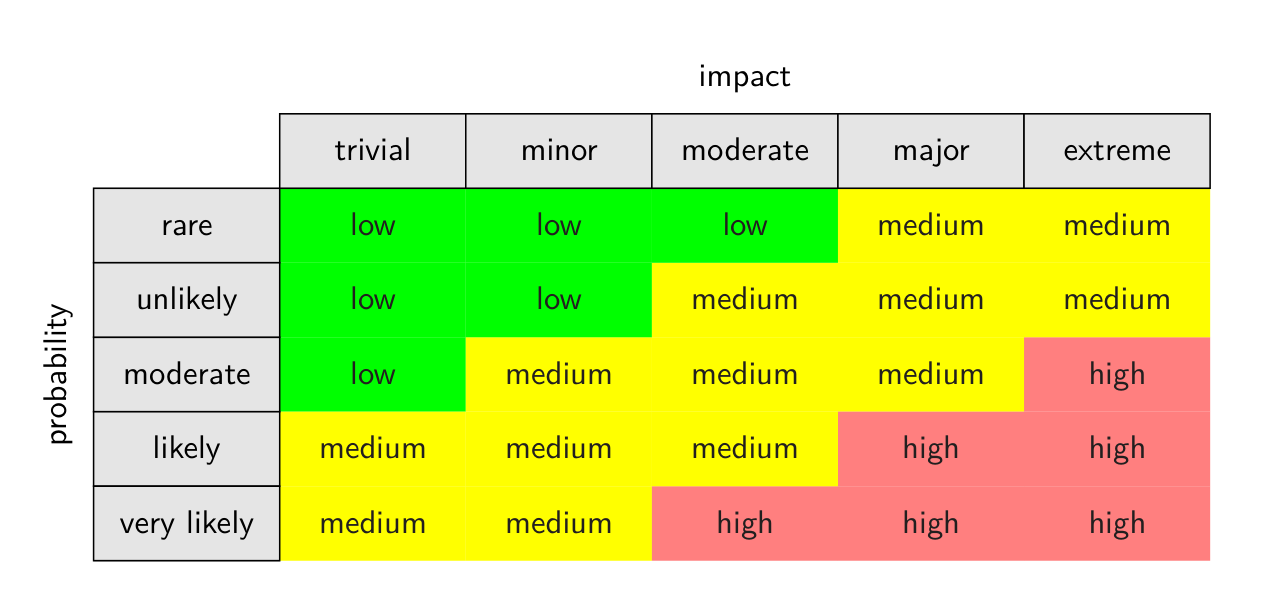
\includegraphics[height=0.35\textwidth]{Figures/Risk Assesment/Qualitative_Matrix.png}
    \caption{Scoring Matrix for Qualitative Risk Analysis.}
\end{figure}

\subsubsection*{Spoofing}
\begin{itemize}
    \item \textbf{ T1 Customer Spoofing }:
        \begin{itemize}
            \item  \textbf{ Bad actor gets Paying Customer account }:

            \begin{itemize}
                \item  \textbf{ Probability }: \textit{Moderate} - Using the same password across different websites is often seen. Given that security measures of those other websites can't be controlled, probability is fairly high and considered as moderate.
                \item  \textbf{ Impact }: \textit{Trivial} - As paying customers are restricted to low-resolution images, these images are deemed non-sensitive. Consequently, any potential leakage of these images would have minimal impact.
                \item \textbf{ Controls in place }: We maintain fairly complete password policies in terms of length, diversity of characters and set up anti-brute force methods like Capchat solving.
                \item \textbf{ Score } : \textit{Low}
            \end{itemize}
            
            \item  \textbf{ Bad actor gets Governmental Customer account }:
            \begin{itemize}
                \item  \textbf{ Probability }: \textit{Moderate} - Justification is the same as previous threat.
                \item  \textbf{ Impact }:  \textit{Major} - Since governmental users have access to sensitive information, images leak is a major concern.
                \item \textbf{ Controls in place }: Same as the previous threat.
                \item \textbf{ Score } : \textit{Medium}
            \end{itemize}
        \end{itemize}
    
    \item \textbf{ T2 IP Spoofing }: 
         \begin{itemize}
                \item  \textbf{ Probability }: \textit{Very Likely} - Given that IP spoofing is utilized in various types of attacks such as man-in-the-middle, DDoS, and botnets, it is reasonable to anticipate that our system will encounter such packets.
                \item  \textbf{ Impact }:  \textit{Major} - If these packets manage to bypass our firewall, it opens up the possibility for an attacker to execute a man-in-the-middle attack.
                \item \textbf{ Controls in place }: Strong firewall policies are set up such that packets incoming from internet with spoofed IP from internal network are refused.
                \item \textbf{ Score } : \textit{High}
        \end{itemize}

    \item \textbf{ T3 Protocol Based Spoofing }:
        \begin{itemize}
            \item  \textbf{ External Protocol Spoofing }:

            \begin{itemize}
                \item  \textbf{ Probability }: \textit{Moderate} - NS spoofing is a common way to get user’s credential leading to our first threat : Customer spoofing.
                \item  \textbf{ Impact }: \textit{Trivial or Major } - Impact depends on the person being spoofed. See Threat 1 : Customer spoofing.
                \item \textbf{ Controls in place }: Use of Secure DNS (DNS SEC) which uses signatures signed with a trusted public key certificate. DNS SEC can prevent DNS cache poisoning.
                \item \textbf{ Score } : \textit{Low to Medium}
            \end{itemize}
            
            \item  \textbf{ Internal Protocol Spoofing }:
            \begin{itemize}
                \item  \textbf{ Probability }: \textit{Unlikely} - Because an attacker must initially execute another form of attack to gain access to the internal network of GASEO. ARP and DHCP packet spoofing threats become less probable.
                \item  \textbf{ Impact }:  \textit{Major} -  Initially, being on the internal network poses a significant concern. Moreover, allowing the potential for a bad actor to execute such attacks could result in information disclosure and other severe consequences.
                \item \textbf{ Controls in place }: Similar to how DNS requests utilize DNSSEC, GASEO employs IDS software that detects ARP spoofing through certification and cross-checking of ARP responses. Any uncertified ARP responses are subsequently blocked.

                For DHCP spoofing, filtering DHCP traffic on concerned ports to/from unknown or untrusted DHCP servers mitigate the risk.
                \item \textbf{ Score } : \textit{Medium}
            \end{itemize}
        \end{itemize}

    \item \textbf{ T4 Physical Spoofing }: 
        \begin{itemize}
            \item  \textbf{ Probability }: \textit{Rare} - Using social engineering to gain physical access requires extensive preparation and poses significant risk for anyone caught in the process. This makes it very  unlikely.
            \item  \textbf{ Impact }:  \textit{Major} - Although physical gaining physical access is unlikely, it makes it easy for a bad actor to deploy other kind of threats that could result in information disclosure, denial of services, tampering, etc.
            \item \textbf{ Controls in place }: Access is restricted through various means such as locked server rooms, physical separation of infrastructure, sign-in sheets, and access cards.
            \item \textbf{ Score } : \textit{Medium}
         \end{itemize}
    
\end{itemize}

\subsubsection*{Tampering}
\begin{itemize}
    \item \textbf{ T5 SQL Injection }: 
        \begin{itemize}
            \item  \textbf{ Probability }: \textit{Likely} -  SQL injection is one of the most common vector of attack regarding web application since user input are often use to make SQL queries.
            \item  \textbf{ Impact }:  \textit{Major to Extreme} - Impact of SQL injection range from major to extreme depending on of the information that has been tampered. A bad actor might tamper with account information to elevate his privileges and gain unauthorized access.
            \item \textbf{ Controls in place }: Sanitizing of every user inputs is strictly required based on the impact that successfully SQL injection could have.
            \item \textbf{ Score } : \textit{High}
         \end{itemize}

    \item \textbf{ T6 Man in the Middle attack }: 
        \begin{itemize}
            \item  \textbf{ Probability }: \textit{Moderate} - Man in the middle attack often occurs on non secure and non secured networks like public WiFi where an attacker could easily intercept traffic.
            \item  \textbf{ Impact }:  \textit{Moderate to Major} - Although governmental customers are required to use trusted networks, there is still a possibility that packets from customers (governmental or not) could be intercepted and tampered to get sensitive data, and privileged access. 
            \item \textbf{ Controls in place }: It's heavily advised for customer to not use public WiFi and to use trusted networks. Furthermore, GASEO websites use HTTPs which encrypt data in transit and verify the identity of the server. Finally multi-factor authentication is used to prevent attackers from impersonating legitimate users.
            \item \textbf{ Score } : \textit{Medium}
         \end{itemize}
\end{itemize}

\subsubsection*{ Repudiation }
\begin{itemize}
    \item \textbf{ T7 Attack on Logs System }: 
        \begin{itemize}
            \item  \textbf{ Probability }: \textit{Likely} -  Attacks on logs are more likely to occur in environments where logs are not properly secured or monitored, or where access controls are weak. Logs represent a primary target for bad actors due to the listing of every action taken.
            \item  \textbf{ Impact }:  \textit{Moderate} - Manipulation on log not only obscures activities of bad actors but also complicates efforts to restore the system in case of more damaging attacks.
            \item \textbf{ Controls in place }: Strong access control, use of hash functions to prevent log tampering and frequent log backup.
            \item \textbf{ Score } : \textit{Medium}
         \end{itemize}
\end{itemize}

\subsubsection*{Information Disclosure}
Since information disclosure is more a consequence than a goal, we will not deal with qualitative risk analysis.

\subsubsection*{Denial of Service}

\begin{itemize}
    \item \textbf{ T9 - T10 Denial of Service attack }:
        \begin{itemize}
                \item  \textbf{ Probability }: \textit{Likely} - DoS attack are very common since their are easey to deploy.
                \item  \textbf{ Impact }:  \textit{Trivial} -  A successful DoS attack can result in the closure of a component within a network infrastructure.
                \item \textbf{ Controls in place }: Use of content delivery netxork (CDN) to redistribute charge in case of DoS attack.
                \item \textbf{ Score } : \textit{Medium}
        \end{itemize}
    
    \item \textbf{ T11 Physical DOS }: 
         \begin{itemize}
                \item  \textbf{ Probability }: \textit{Rare} - Using social engineering to gain physical access requires extensive preparation and poses significant risk for anyone caught in the process. This makes it very  unlikely.
                \item  \textbf{ Impact }:  \textit{Extreme} -  Although obtaining physical access for a DOS attack may seem excessive, the impact on the system could be severe, as malicious actors could potentially damage expensive equipment GASEO heavily relies on. The EO data feed and servers are likely to be primary targets.
                \item \textbf{ Controls in place }: Access is restricted through various means such as locked server rooms, physical separation of infrastructure, sign-in sheets, and access cards.
                \item \textbf{ Score } : \textit{Medium}
        \end{itemize}
\end{itemize}

\subsubsection*{Escalation of Privilege}
Since escalation of privileges is more a goal than a type of attacks, we will not deal with qualitative risk analysis.

\subsubsection*{Scoring Matrix Placement}
Here's the placement of previous threats on the Scoring Matrix :
\begin{figure}[h]
    \centering
    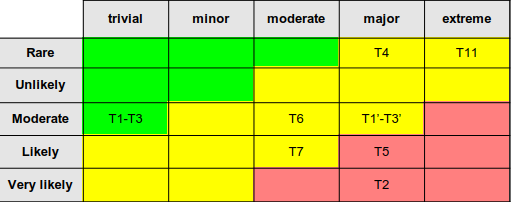
\includegraphics[height=0.20\textwidth]{Figures/Risk Assesment/Qualitative_Matrix2.png}
    \caption{Scoring Matrix for Qualitative Risk Analysis.}
\end{figure}

\newpage

\subsection{ Quantitative Risk Analysis }
Based on the following tables and scoring matrices, we will determine frequency and capability of previous threats:
\begin{figure}[h]
    \centering
    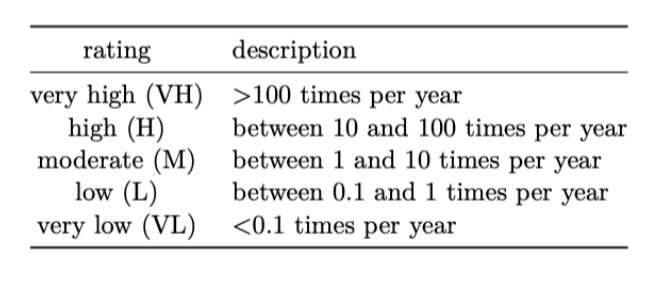
\includegraphics[width=0.49\textwidth]{Figures/Risk Assesment/Threat_Event_Freq.png}
    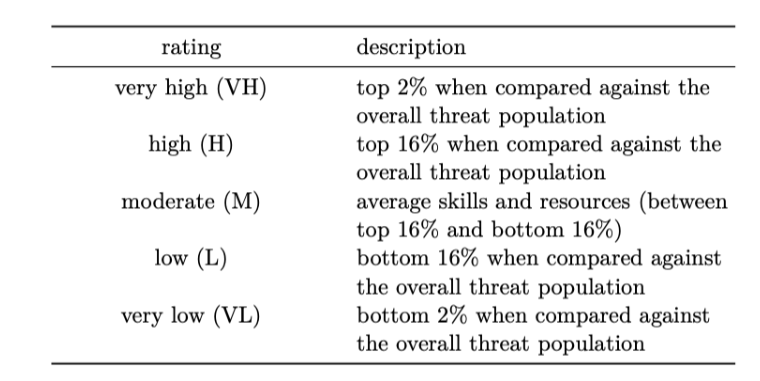
\includegraphics[width=0.49\textwidth]{Figures/Risk Assesment/Threat_Capcacity.png}
    \caption{Threat event frequency and threat capacity.}
\end{figure}

\begin{figure}[h]
    \centering
    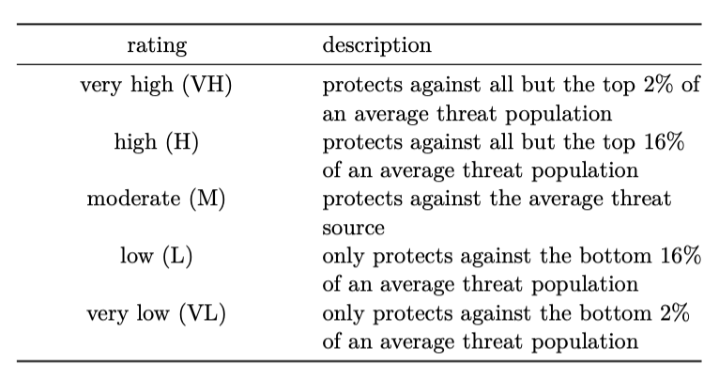
\includegraphics[width=0.49\textwidth]{Figures/Risk Assesment/Threat_Control_Str.png}
    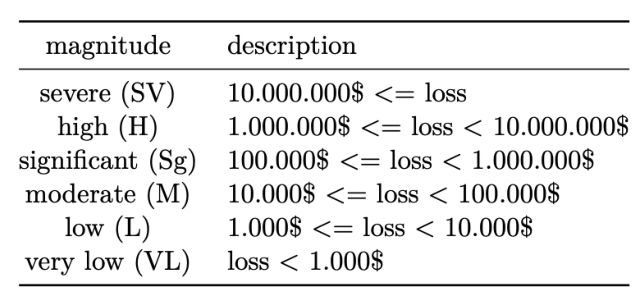
\includegraphics[width=0.49\textwidth]{Figures/Risk Assesment/Threat_Loss.png}
    \caption{Threat control Strength and probable loss magnitude.}
\end{figure}


\begin{figure}[h]
    \centering
    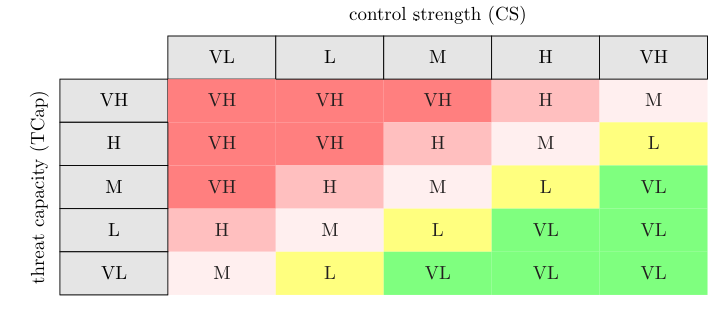
\includegraphics[width=0.32\textwidth]{Figures/Risk Assesment/Threat_vunl_mat.png}
    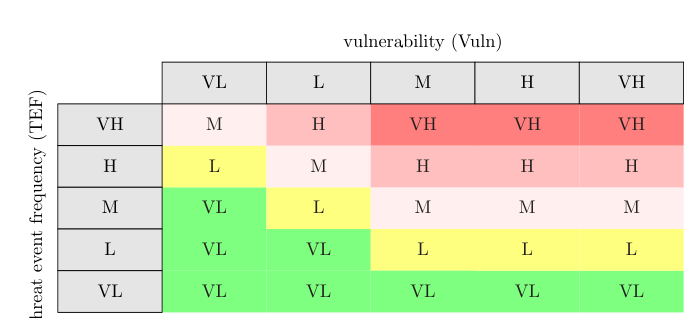
\includegraphics[width=0.32\textwidth]{Figures/Risk Assesment/Threats_loss_mat.png}
    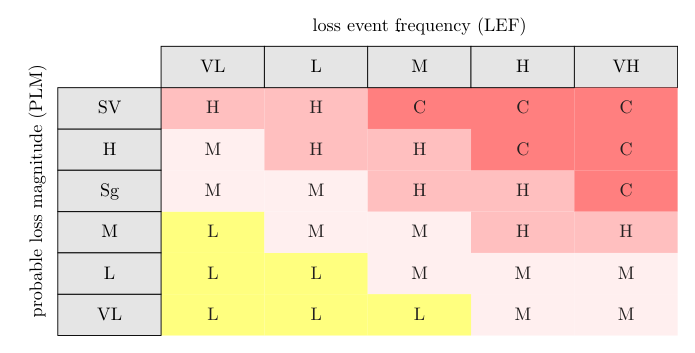
\includegraphics[width=0.32\textwidth]{Figures/Risk Assesment/Threat_risk_mat.png}
    \caption{Vulnerability matrix, Lost event frequency matrix and risk magnitude matrix.}
\end{figure}

\newpage

\subsubsection*{ Denial of Service }
\begin{itemize}
    \item \textbf{ T9 Websites Denial of Services}: 
        \begin{itemize}
            \item  \textbf{ Threat Event Freq. }: \textit{High} - Since DDOS attack are very frequent and easy to deploy, it is assumed that the \textbf{TEF} is high.
            \item  \textbf{ Threat Capacity }: \textit{Low} - DDOS attack are frequent, easy to deploy and does not grant anything other thant non working infrastructure. It is fair to assume that DDOS attack would be in the bottom 16\% in term of \textbf{TC}. 
            \item  \textbf{ Threat Control Strength }: \textit{Very High} - DDOS attacks are unsophisticated and only require Control Delivery Networks to redistribute traffic and mitigate the attack. It is then assume that the \textbf{TCS} is very high
            \item  \textbf{ Probable loss magnitude }: \textit{Significant} - Based on some researches, \textbf{PLM} is determined by : $\text{PLM} = \text{TEF} \times \text{TC} \times \text{TCS} \times \text{AV}$ with \textbf{AV} asset value. Let says our websites assets values are 10k€ we can assume that PLM would be $10 \times 2 \times 5 \times 10.000 $  which makes it significant for \textbf{PLM}
         \end{itemize}
\end{itemize}

Based on the previous matrices, we establish that Website Denial of Service is classed as :
\begin{itemize}
    \item \textbf{ Vulnerability } : \textit{Very Low} -  Based on vulnerability matrix, by taking threat capacity and threat control strength.
    \item \textbf{ Lost Event Frequency } : \textit{Low} - Based on lost event frequency matrix, by taking vulnerability and threat event frequency.
    \item  \textbf{ Risk magnitude } : \textit{Medium} - Based on risk magnitude matrix, by taking lost event frequency and probable loss magnitude.
\end{itemize}
\newpage
%~~~~~~~~~~~~~~~~~~~~~~~~~~~~~~~~~~~~~~~~~~~~~~~~~~~~~~~~~~~~~~~~~~~~~~~~~~~~~~~~~~~~~~~~~~~~~~~

\section{Risk Treatment}\label{Sec: Treatment}

In addition to all proposed risk treatments,we assume ongoing constant monitoring and logging across various network levels.

\subsection{Spoofing}
\begin{itemize}
    \item \textbf{T1 Customer Spoofing} - \textit{Low to Medium} : Maintain fairly complete password policies in terms of length, diversity of characters and set up anti-brute force methods like Capchat solving.

    Strong authentication methods such as two-factor authentication are used to connect to GASEO's infrastructure.
    \item \textbf{T2 IP Spoofing} - \textit{High} : Strong firewall policies are set up such that packets incoming from internet with spoofed IP from internal network are refused.
    \item \textbf{T3 Protocol Based Spoofing} - \textit{Low to Medium} : Use of Secure DNS (DNSSEC) which uses signatures signed with a trusted public key certificate. DNSSEC can prevent DNS cache poisoning.

    Use of static IP addresses for critical devices whenever possible to reduce reliance on DHCP and mitigate the risk of DHCP spoofing.
    
    Use of static ARP entries on critical devices to explicitly define MAC-to-IP address mappings. This prevents attackers from successfully poisoning the ARP cache with false mappings. For non critical devices use of IDS software that detects ARP spoofing through certification and cross-checking of ARP responses. 

    \item \textbf{T4 Physical Spoofing} - \textit{Medium} : Restriction of access in various means such as locked server rooms, physical separation of infrastructure, sign-in sheets, and access cards. 
\end{itemize}

\subsection{Tampering}
\begin{itemize}
    \item \textbf{T5 SQL Injection} - \textit{High} : In term of best coding practices 
        \begin{itemize}
            \item Sanitizing of every user inputs.
            \item Database is granting users the minimum privileges necessary to perform their tasks.
            \item Use of secure coding frameworks and libraries that offer built-in protections against SQL injection.
        \end{itemize}
    In term of infrastructure : 
        \begin{itemize}
            \item Use of web application firewall (WAF) capable of detecting and blocking SQL injection attacks in real-time by analyzing incoming HTTP requests and responses, identifying and filtering out malicious SQL injection payloads.
        \end{itemize}
        
    \item \textbf{T6 Man in the Middle Attack} - \textit{Medium} : Use of encryption protocols such as HTTPS/TLS for securing communications over networks.

    Validation of SSL/TLS certificates presented to ensure they are issued by trusted Certificate Authorities.

    Use of multi factor authentication to prevent further spoofing.
\end{itemize}

\subsection{Repudiation}
\begin{itemize}
    \item \textbf{T7 Attack on Logs Systems} - \textit{Medium} : Use dedicated logging servers or services with restricted access to authorized personnel.

    Use of hash functions and storage of log data in immutable storage solutions to prevent retroactive tampering or deletion of log entries by malicious user.

    Frequent log backup and redundancy of data.
    
\end{itemize}

\subsection{Information Disclosure}
\begin{itemize}
    \item \textbf{T8 Various Leaking Methods} : Use of encryption for full disk, database and email to protect sensitive data from unauthorized access or interception.

    Restriction of access in various means such as locked server rooms, physical separation of infrastructure, sign-in sheets, and access cards. 
\end{itemize}

\subsection{Denial of Service}
\begin{itemize}
    \item \textbf{T9 - T10 Websites DOS} - \textit{Medium} : Use of content delivery network (CDN) to redistribute charge across multiple servers.

    Use of Client Puzzle Protocol (CPP) which establish a connection only if the client has resolved a mathematical puzzle.

    Blacklist of specific ip addresses known for Dos attack.
    \item \textbf{T11 Physical DOS} :  - \textit{Medium} : Restriction of access in various means such as locked server rooms, physical separation of infrastructure, sign-in sheets, and access cards. 
\end{itemize}





\newpage
%~~~~~~~~~~~~~~~~~~~~~~~~~~~~~~~~~~~~~~~~~~~~~~~~~~~~~~~~~~~~~~~~~~~~~~~~~~~~~~~~~~~~~~~~~~~~~~~
\section{Solutions}\label{Sec: Solutions}

\subsection{Meta Policies}

It's important to note that we have segmented our information domain as such:
\begin{itemize}
    \item \textit{"public internet"} - \textit{"administration information"} - \textit{"EO proc. Software"} - \textit{"EO Data"}
\end{itemize}

\subsubsection*{Confidentiality}
In our case, it is clear that confidentiality takes precedence over data integrity. 
We establish that everything related to EO must be considered as a CONFIDENTIAL level of confidentiality since satellites images provided are sensible information. Administration should have a classic level of confidentiality hence the RESTRICTED level. Finally all that is public is by default related to UNCLASSIFIED.

\begin{figure}[h]
    \centering
    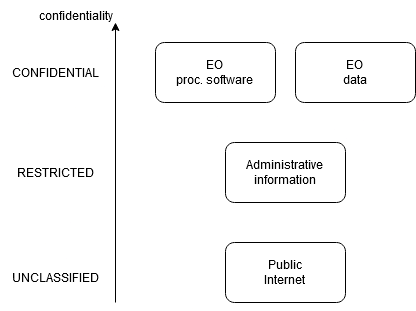
\includegraphics[width=0.35\textwidth]{Figures/Solutions/classification_conf.png}
    \caption{Confidentiality of segmented information domain.}
\end{figure}

As confidentiality is a very high priority, the BellaPadula (\textbf{BLP}) meta-policy will be enforced. Such policy implies two simple rules : 
\begin{itemize}
    \item \textit{No read up} : a subject (a user or a process) with a certain security clearance level cannot read data at a higher security level unless authorized to do so. It prevent unauthorised user to get access to confidential information.
    \item \textit{No write down} :  a subject with a certain security clearance level cannot write (or transfer) data to a lower security level. This prevents the unauthorized disclosure of sensitive information.
\end{itemize}

To effectively implement the BLP policy within our system, we must establish a multi-level security (MLS) for the various data objects, assigning each a confidentiality level and corresponding labels.

For the Confidentiality we establish 4 levels ranking as such : 
\begin{itemize}
    \item \textbf{Unclassified} : \textit{\textbf{Non}-downloaded low-resolution images} present on the public website - Since this data is publicly available it is considered as unclassified.
    \item \textbf{Restricted} : \textit{Downloaded low-resolution images } - The act of downloading an image requires password protection, making it as restricted access.
    \item \textbf{Confidential} : \textit{High-resolution images} - These images are only accessible to governmental agencies and will require added security measures like encryption.
    \item \textbf{Secret} : \textit{Reports of geographical zones} - These comprehensive reports may pertain to military zones, restricted areas, etc. Therefore, it's essential to classify them as secret.
\end{itemize}

For the labels we have : 
\begin{itemize}
    \item \textit{Public} - \textit{Governmental} - \textit{Military} - \textit{Reports} - \textit{Low Resolution} - \textit{High Resolution}
\end{itemize}

\subsubsection*{Integrity}
Like it has been said before, everything EO related will emphasise confidentiality rather than integrity hence the LOW INTEGRITY level of EO proc. Software and EO data. 
\begin{figure}[h]
    \centering
    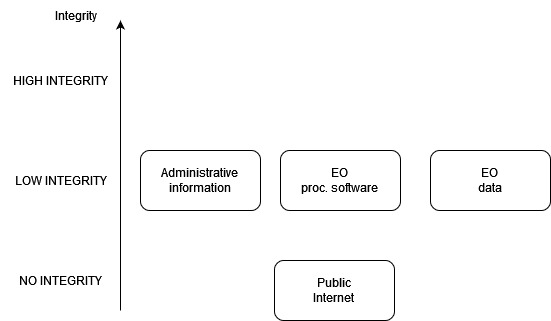
\includegraphics[width=0.35\textwidth]{Figures/Solutions/classification_integ.png}
    \caption{Integrity of segmented information domain.}
\end{figure}

Since images that are processed are still confidential but with low integrity, it is important to implement \textbf{Least Privilege} principle which implies that users and processes should still be granted the minimum level of access necessary to perform their tasks. This principle reduces the risk of accidental or intentional misuse of information.

\newpage
\subsubsection*{Network Topology}

\begin{figure}[h]
    \centering
    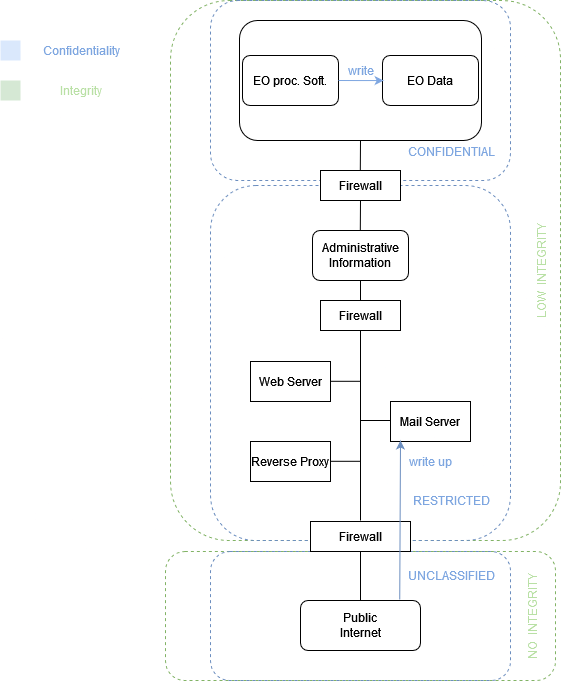
\includegraphics[width=0.8\textwidth]{Figures/Solutions/network_topology.png}
    \caption{Integrity of segmented information domain.}
\end{figure}

\newpage

\subsection{Additional policies}
In addition to the meta policies, we can apply more specific policies to improve the security of GASEO :

\subsubsection*{User's policies}
As mentioned earlier regarding integrity preservation, it is good practice to apply the principle of \textbf{least privilege}, granting users, customers, and internal personnel only the necessary level of access to perform specific tasks. This approach is typically paired with the \textbf{zero trust} concept, where no trust is assigned to an individual based on attributes like network location or name. \textbf{Role Based Access Control (RBAC)}is therefore applied with \textbf{Multi Factor Authentication (MFA)}.

\subsubsection*{Infrastructure policies}
In terms of infrastructure, we are constantly \textbf{updating} our systems and \textbf{applying patches}. This type of modification is first carried out on a test infrastructure and then deployed at the appropriate level. Patches are applied in accordance with a \textbf{regular risk assessment}.

To assist with ongoing risk assessment, a range of \textbf{firewall}, \textbf{intrusion detection systems (IDS)} and \textbf{anti viruses} are set in place. A penetration testing team can be engaged to test the reliability of our systems and a set of physical security standards are applied.

\subsubsection*{Data Storage, Data Exchange and Network policies}

Regarding data storage and data exchange the watchword is \textbf{encryption}. In idle time, data is stored and encrypted using a strong algorithm such as \textbf{AES-256}.
In transit, the same data is relayed over the network using protocols that also enable encryption, such as \textbf{TLS/SSL}.

Finally, since governmental users work with data ranging from confidential to secret in terms of confidentiality, any exchange of such data must use an \textbf{public encryption scheme} with public and private keys to guarantee the integrity of the data during transfer and also the impossibility of using the data in the event of loss. 

\subsection{Building Blocks}

\subsubsection*{Phishing email protection}
One effective method to directly mitigate \textbf{T1} is to implement a machine learning-based phishing email protection system. While this solution is highly specialized, it can also help prevent other types of threats, such as \textbf{T6}, \textbf{T7}, \textbf{T8}, and \textbf{T10}, by blocking emails with attached malware.

\subsubsection*{Network Segmentation}
A well-implemented network segmentation can often limit attack surface, further enhance our BLP meta-policies and help role based access control ensuring confidentiality and integrity. This is generally done with router, switches and firewall and in our case we will implement the following : 
\begin{itemize}
    \item \textbf{Additional Firewall} : A third firewall is added to separate the EO data processor, EO server, and EO data feed. Additionally, backup servers and log servers, which require a high level of integrity, will be included. It is important to note that some serve will stay in the 3rd part and some in the 4th based on their importance. This process is illustrated with Figure 
     \ref{fig:firewall_nat}.
    \item \textbf{NAT} : Network Address Translation (NAT) protocol is implemented for each LAN (office LAN and Tech LAN). This protocol aids in obfuscating workstations, making it difficult for a bad actor to determine the network topology and gain direct access. Additionally, it facilitates scaling in alignment with GASEO's growth.
    \item \textbf{Additional LAN} : Since a new level has been added to the network topology, an additional LAN need to be added to maintain confidentiality. 
\end{itemize}

With this segmentation, threats \textbf{T2 - T3 - T7 - T8 - T9 - T10 - T12}

\begin{figure}[h]
    \centering
    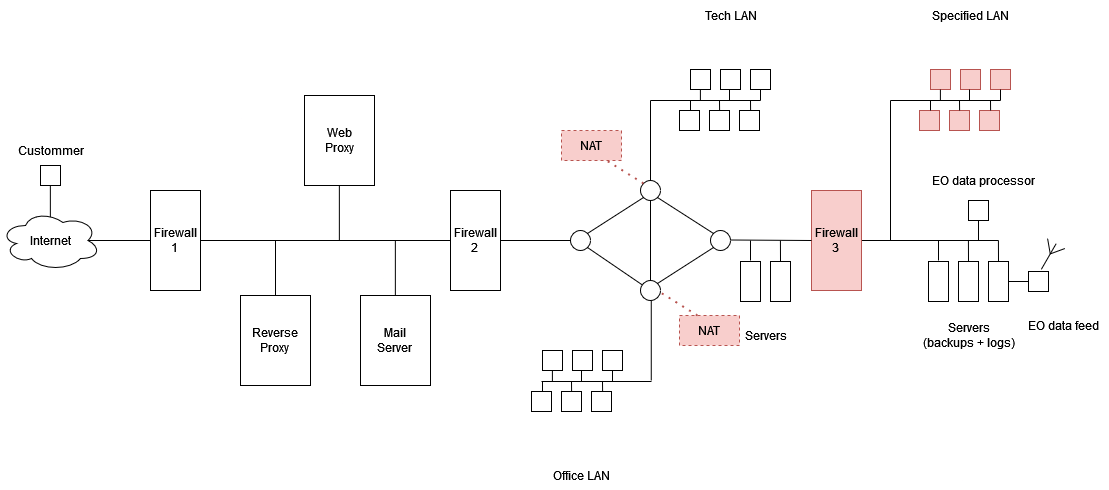
\includegraphics[width=0.75\textwidth]{Figures/Solutions/firewall_nat_lan.png}
    \caption{Network Segmentation.}
    \label{fig:firewall_nat}
\end{figure}

\newpage
\subsubsection*{Web Application Firewall (WAF)}
A Web Application Firewall (\textbf{WAF}) is designed to prevent and mitigate various types of attacks targeting web application by filtering, monitoring, and blocking HTTP suspicious traffic to and from a web service. It directly prevent \textbf{T5} and help mitigate \textbf{T2 - T9 - T10}. In our case it will be set up just behind the first firewall to analyse request performed to our reverse proxy.

\subsubsection*{Intrusion Detection System (IDSs)}
An intrusion detection system \textbf{IDS} is a device or software application that monitors a network or systems for malicious activity or policy violations. Its a passive component of the  topology and help mitigating nearly all threats but the physical one.

We differentiate between Host-based Intrusion Detection Systems (HIDS) and Network-based Intrusion Detection Systems (NIDS), which analyze different aspects of a computing environment.\textbf{HIDS} monitors and analyzes the internals of a computing system, such as system logs, file integrity, and user activities. In contrast,\textbf{NIDS} examines network traffic, inspecting data packets that travel across the network for suspicious activity and.

In our case IDS are set up as such : 
\begin{itemize}
    \item \textbf{IDS 1 (NIDS)} : Monitors traffic coming from the internet after it passes through Firewall 1. It detects any malicious traffic that might have bypassed the firewall and targets internal services of the DMZ. It ensures that malicious activities are caught early.
    \item \textbf{IDS 2 (NIDS)} : Monitors internal network traffic between different segments (Office LAN, Tech LAN). It detects lateral movement of threats within the internal network and help in the mitigation of malware propagation.
    \item \textbf{IDS 3 (HIDS)} : Monitors activities on these specific servers, such as file integrity, process activity, and user actions. It ensures that unauthorized access or changes are detected and provides detailed monitoring and protection for critical servers. Although it might generate many false positives, the critical nature of this network segment necessitates the use of a machine learning-based IDS.
\end{itemize}

\begin{figure}[h]
    \centering
    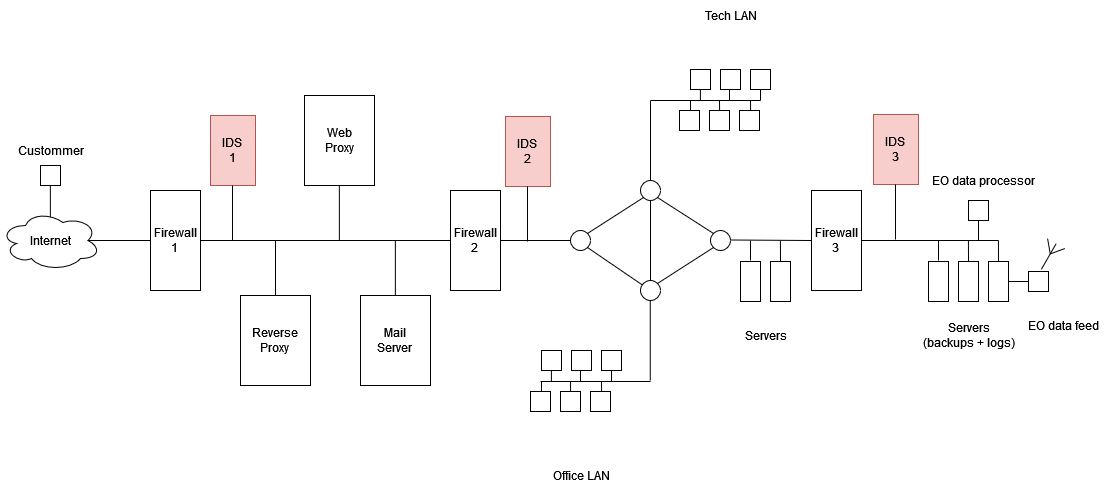
\includegraphics[width=0.75\textwidth]{Figures/Solutions/network_topo_ids.png}
    \caption{Addition of IDS in the network topology.}
\end{figure}


\subsubsection*{VPN}
When accessing GASEO infrastructure remotely, Virtual Private Network (VPN) provides a secure way for authorized external users to connect to sensitive data and applications, shielding them from potential risks present on the public internet.
It directly prevent \textbf{T1 - T2 - T6} which often occur in data stealing on non secure channel of communication by encrypting it. A local VPN server can be installed within the network topology. 

\subsubsection*{Backup Server}
Backup systems are an essential part of security management within a company. Although their applications do not actively prevent/mitigate a potential threat, they enable a system to be redeployed relatively quickly in the event of a major incident. 
Because of its recovery nature, the backup system is critical in terms of integrity (just like the log system) and requires relatively high levels of isolation (see fig \ref{fig:firewall_nat}). This is why, in our topology, the backup system is located in the EO data feed section.
To mitigate the risk of data loss, frequent back up policies on critical system like ED and logs need to be applied.
\subsubsection*{Log System}
While the logging system may not be the most dynamically active component of a security infrastructure, its significance in recovery and forensic analysis cannot be overstated. Similar to backup systems, logging must be implemented at every level with utmost integrity, warranting their isolation within network topology (see fig \ref{fig:firewall_nat}). Encryption should be applied to storage, and adherence to strict role-based access controls is imperative.

\newpage
\subsection{Certified Product}
While developing a custom VPN solution seems better for specific needs, it can also be a lot of work and not comply with safety standards in application. GASEO therefore decided to use \textbf{Cisco AnyConnect Secure Mobility Client} \footnote{\url{https://www.cisco.com/c/en_uk/products/security/anyconnect-secure-mobility-client/index.html}} product to make it cost and resource efficient while granting \textbf{FIPS 140-2} and \textbf{Common Criteria (CC)} \footnote{\url{https://www.commoncriteriaportal.org/files/epfiles/st_vid11289-ci.pdf}} certification.

\begin{figure}[h]
    \centering
    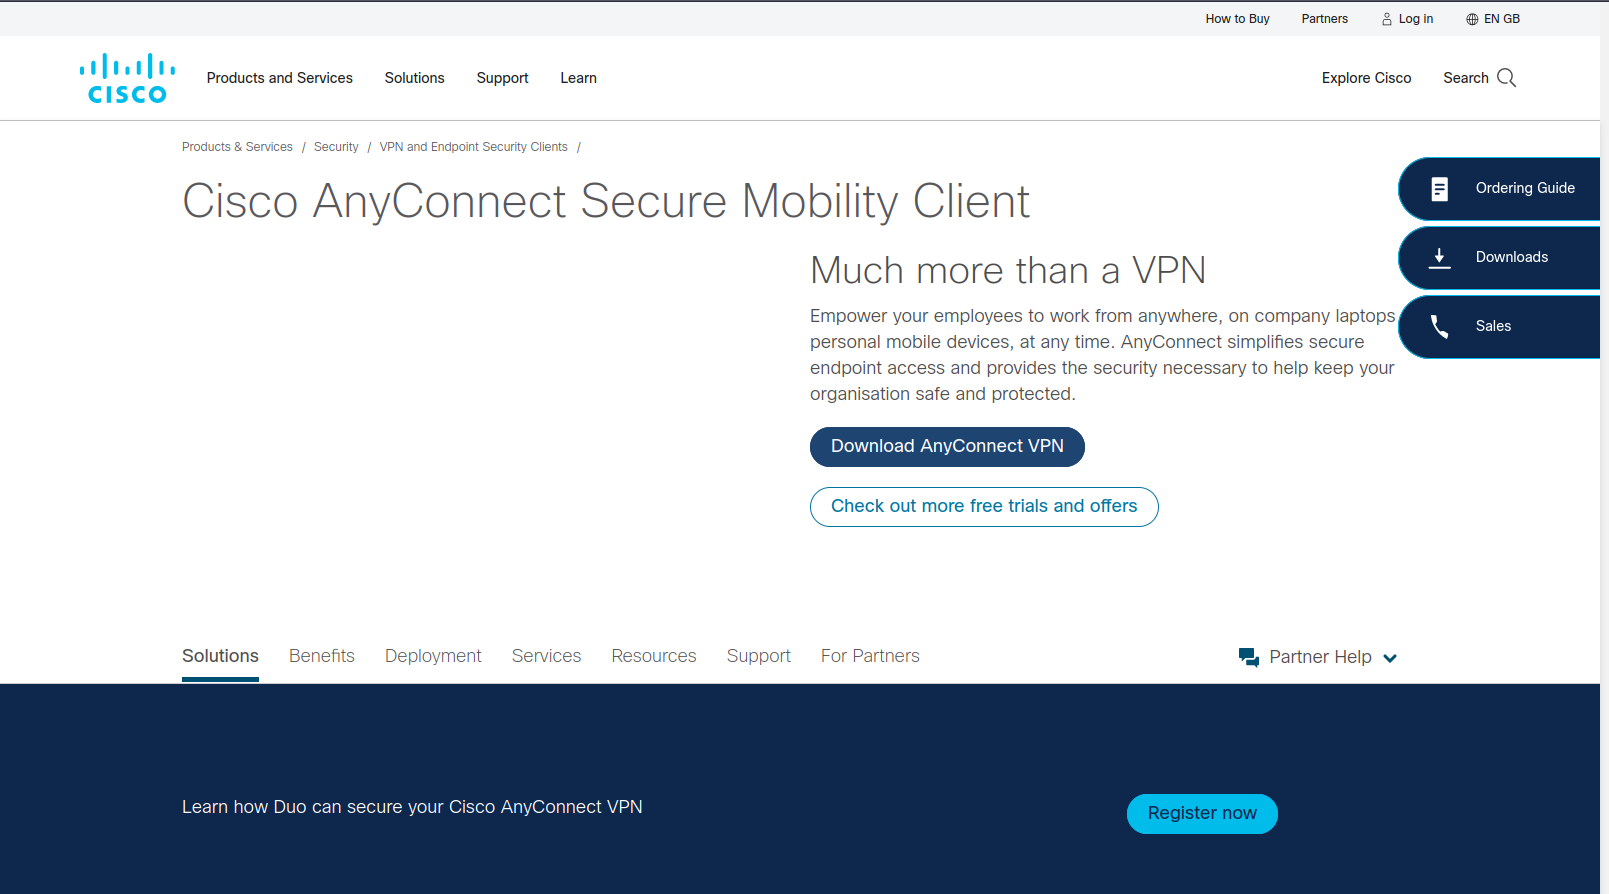
\includegraphics[width=0.75\textwidth]{Figures/Solutions/cisco_vpn.png}
    \caption{Cisco AnyConnect product page.}
\end{figure}

\textbf{FIPS 140-2} certification named \textit{Security Requirements for Cryptographic Modules} and was issued by NIST. IT  is a U.S. government standard that specifies the security requirements for cryptographic modules used to protect sensitive information. 
Althoug it was last issued in decembre 2002, it's relevance come from the fact that it ensures robust encryption and data protection needed by a VPN and crucial for defending against sophisticated threat.

Based on the Cisco Ordering guide\footnote{\url{https://www.cisco.com/c/en/us/products/collateral/security/anyconnect-secure-mobility-client/secure-client-og.html}} of \textbf{Cisco AnyConnect Seure Mobility Client} : \textit{"The Cisco Secure Client consistently raises the bar by making the remote-access experience easy for end users while providing the security that enterprise IT requires. It helps enable a highly secure connectivity experience across a broad set of PC and mobile devices. As mobile workers roam to different locations, they automatically resume connectivity. The always-on intelligent VPN adapts the tunneling protocol to the most efficient method, such as the Datagram Transport Layer Security (DTLS) protocol for latency-sensitive VoIP traffic or TCP-based application access. Tunneling support is also available for IP Security Internet Key Exchange version 2 (IPsec IKEv2)."}

\newpage
%~~~~~~~~~~~~~~~~~~~~~~~~~~~~~~~~~~~~~~~~~~~~~~~~~~~~~~~~~~~~~~~~~~~~~~~~~~~~~~~~~~~~~~~~~~~~~~~
\section{Resilience}\label{Sec: Resilience}

Cyber resilience refers to an agency ability to continuously deliver services under pressure like cyber attack. It can be applied to software and hardware ranging from a simple application to a general wide system agency.

GASEO has implemented several measures that align with the five pillars of cyber resilience. However, there are opportunities for improvement in each area to enhance the overall resilience of the system. By adopting these improvements, GASEO can better protect against, detect, respond to, and recover from cyber threats, ensuring the continuity and security of its services.

\subsection{Five pillars of Cyber Resilience}
\begin{figure}[h]
    \centering
    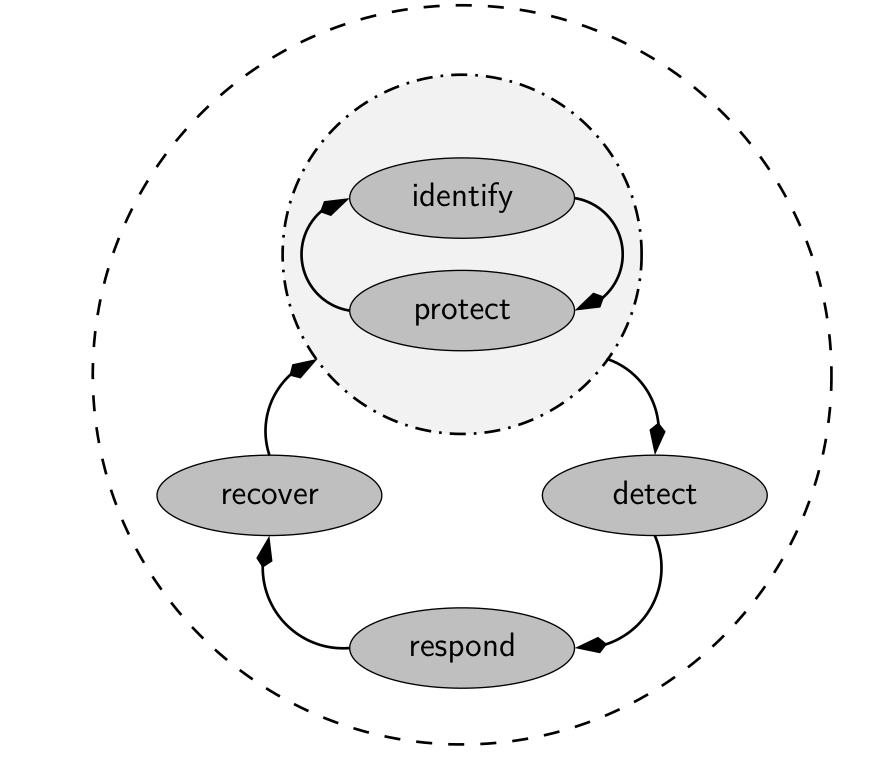
\includegraphics[width=0.35\textwidth]{Figures/Resilience/resilience-five_pillar.png}
    \caption{Five pillar of resilience.}
\end{figure}

\subsubsection*{Identify}
GASEO's approach to identifying risks and vulnerabilities includes a risk assessment process which involves both qualitative and quantitative risk analyses that consider various threats. 

However such risk assessment must be relevant at any time and evolve to better correspond modern threats. This is why GASEO should perform regular security audit either based on :
\begin{itemize}
    \item \textbf{Basic time schedule} : Every 3 to 6 month, GASEO perform a similar assessment on its infrastructure.
    \item \textbf{Threat intelligence} : GASEO could adapt its risk management policies based on data gathering from various source such as other industry security reports, security vendors, cybersecurity events.
\end{itemize}
To carry out such regular checks, it is important to have competent, well-trained personnel. GASEO could also employ third parties to carry out risk assessments on smaller, less confidential infrastructures such as the demilitarized zone.

\subsubsection*{Protect}
GASEO's current protection measures include the application of cryptographic algorithms to data transfer and storage, multi-factor identification, network segmentation to limit the propagation of an attack, role based access control an zero trust model.

To help ensure better protection, GASEO can perform automated scans using tools such as OpenVAS to identify and patch vulnerabilities directly, and engage a pentesting team to test the reliability of the infrastructure. 

Finally, even if these policies are already in force. GASEO can extend the zero-trust principle to all network devices, and implement Identity Access Management to guarantee stricter access control.

\subsubsection*{Detect}
GASEO has implemented IDS at every level of its network, varying from NIDS to HIDS. These detection systems are passive and enable constant monitoring of the network and its hosts sometimes based on machine learning.

However, the passivity of such a system can be criticized. It's probably better to replace the first two NIDS with Network Intrusion Prevention System or NIPS, enabling action to be taken in the event of suspicious activity.
It is important to note that the HIDS of the critical section must not be changed to HIPS to avoid the possibility of facilitating a DOS attack.

In term of \textbf{SWOT analysis} : 
\begin{itemize}
    \item \textbf{Strengths} : \textit{Diversity within the analysis equipment} - GASEO has put in place a set of HIDS and NIDS providing an approach covering both networks and hosts in topologically relevant areas.
    \item \textbf{Weaknesses} : \textit{Limited anomaly detection} - IDSs can generate a large number of false positives. Especially when they are ML based. In addition, such systems do not necessarily have the capacity to detect more specialised threats such as 0-day attacks, which by definition do not correspond to any known signature.
    \item \textbf{Opportunities} : \textit{Automation and Machine Learning} - With the development of machine learning, GASEO can improve its ability to detect paterns that were previously too complex to express ‘manually’. It is also possible to automatically update these paterns more frequently to keep abreast of the latest threats.
    \item \textbf{Threats} : \textit{Evolving threats and attackers} - Cyber attacks are constantly evolving and increasingly bypassing detection systems. Combined with a limit on both technological and monetary resources, the aim is to maintain up-to-date knowledge of the latest threats and adapt the strategies in place.
\end{itemize}


\subsubsection*{Respond}
GASEO has implemented a risk treatment plan, however it may be interesting to develop in parallel a Detailed Incident Playbooks which provide specific and detailed guidance of a threat to ensure a consistent and measured response. To assist in a better response a team can be trained using these guidelines and authorized to conduct incident response on a similar system or on the main GASEO system.

\subsubsection*{Recover}
GASEO has a high integrity backup system.However, a sufficient frequency must be ensured.

In addition, separating the backup system from the network, or even from an off-site network, can help in the event of a threat to the said system.
Finally, GASEO could invest in Disaster Recovery as a Service (or DRaaS), a cloud computing service, which provides faster recovery times and reduce downtime following an incident.


\subsection{ISO 27000}
The ISO 27000 family of standards provides guidelines and best practices for information security management systems (ISMS). It helps organizations manage the security of assets like financial information, intellectual property, employee details, and information entrusted by third parties. The key standard, ISO/IEC 27001, outlines requirements for establishing, implementing, maintaining, and continually improving an ISMS.

The ISO/IEC 27001 define four step wich applied to GASEO give : 
\begin{itemize}
    \item \textbf{Scope Definition} : Involves defining the boundaries and context of the ISMS by identifying which parts of the organization and what types of information will be included and understanding the internal and external issues that can impact said ISMS. This step is illustrated in section \ref{Sec: Context}
    \item \textbf{Asset Inventory} : Involves identifying and documenting all information assets that are within the scope of the ISMS. An information asset can be any data, device, or other component that supports information-related activities. This step is illustrated in the section \ref{Sec: Processes}.
    \item \textbf{Risk Assessment} : Is the process of identifying, analyzing, and evaluating risks to the organization's information assets. This helps to understand the potential threats, vulnerabilities, and impacts on the organization. This process is illustrated in the section \ref{Sec: Assessment}.
    
    \item \textbf{Risk Treatment} :  Involves selecting and implementing measures to mitigate, transfer, avoid, or accept the identified risks. The goal is to reduce risks to an acceptable level in alignment with the organization's risk appetite and objectives. This process is illustrated in the section \ref{Sec: Treatment} and \ref{Sec: Solutions}. 
\end{itemize}

In summary, the various stages of the ISO 27001 standard are illustrated throughout this project. However, in order to comply with the standard, it is necessary to repeat the whole process every redefined period of time.

\subsection{NIST CSF 2.0 SP1300}

\subsubsection*{Governance}
 \begin{itemize}
     \item \textit{As our business grows, how often are we reviewing our cybersecurity strategy?}
     
     - GASEO should establish a regular review cycle for its cybersecurity strategy quarterly ensuring it stays updated with the latest threats and regulatory changes.
    
     \item \textit{Do we need to upskill our existing staff, hire talent, or engage an external partner
to help us establish and manage our cybersecurity plan ?}

    - GASEO should consider a mix of upskilling existing staff continuously trained and hiring specialized talent. Additionally, engaging external partners for specific tasks like penetration testing can provide a more robust cybersecurity posture. Risk assessment should be let to GASEO since some information might be concidered confidential or secret.
     \item \textit{Do we have acceptable use policies in place for business and for employee-owned
devices accessing business resources? Have employees been educated on these
policies?} 
    - GASEO should implement strict use policies for company-owned accessing the network. Personal devices should be limited or banned for limiting data leak. In return, GASEO provides its employees with all the equipment needed for a typical job. Regular training and awareness programs should be conducted to ensure employees are familiar with these policies.
 \end{itemize}

\subsubsection*{Identify}
 \begin{itemize}
     \item \textit{What are our most critical business assets (data, hardware, software, systems, facilities, services, people, etc.) we need to protect?}

    \begin{itemize}
        \item \textbf{Data} : High resolutions images, customer data.
        \item \textbf{Hardware} : Servers, workstations, and networking equipment.
    \end{itemize}
    
     \item \textit{What are the cybersecurity and privacy risks associated with each asset?} 

    \begin{itemize}
        \item \textbf{Data} : Risk of data breaches leading to loss of customer trust and leak of military grade images.
        \item \textbf{Hardware} : Physical theft or damage could result in data loss and operational downtime.
    \end{itemize}
     
     \item \textit{What technologies or services are personnel using to accomplish their work? Are these services or technologies secure and approved for use?}

     - In term of technologies, all devices usefull to GASEO task are given by GASEO granting security and approval. For the services, employees can use  Cloud storage, email services, and collaboration tools that only come  from a contract between GASEO and a recognised company like Microsoft (for Office365, Microsoft Teams, etc.). 
     
 \end{itemize}

\subsubsection*{Protect}
 \begin{itemize}
     \item \textit{Are we restricting access and privileges only to those who need it? Are we removing access when they no longer need it?}
     
     - GASEO enforce no trust model, least privilege principle and role base access control. No one should have more access or rights than required for a specific task at any time.
     
     \item \textit{How are we securely sanitizing and destroying data and data storage devices when they’re no longer needed?}
     
     - GASEO should follow a strict data sanitization policy that includes data wiping, degaussing, and physical destruction of storage devices to ensure that data cannot be recovered.
     
     \item \textit{Do employees possess the knowledge and skills to perform their jobs with security in mind?}
     
     - GASEO employees receive regular cybersecurity training, including phishing awareness, secure password practices, and data handling protocols.
 \end{itemize}

\subsubsection*{Detect}
 \begin{itemize}
     \item \textit{Do devices that are used for our business, whether business-owned or employee-owned, have antivirus software installed?}
     
     - All devices used for business purposes are equipped with up-to-date antivirus software. Regular scans and updates are enforced to maintain security.
     
     \item \textit{Do employees know how to detect possible cybersecurity attacks and how to report them?}
     
     - Employees are trained to recognize signs of cybersecurity attacks, such as phishing emails and unusual system behavior. A clear reporting protocol is in place for them to follow.
     \item \textit{How is our business monitoring its logs and alerts to detect potential cyber incidents?}
     
     - GASEO uses a system of IDSs and Logs to monitor logs and alerts. The system is configured to detect anomalies and generate real-time alerts for potential cyber incidents.
 \end{itemize}
 
\subsubsection*{Respond}
 \begin{itemize}
     \item \textit{Do we have a cybersecurity incident response plan? If so, have we practiced it to see if it is feasible?}
     
     - GASEO has a comprehensive incident response plan, which is reviewed and tested regularly through simulated cyber attack exercises. This is illustrated in section \ref{Sec: Treatment}
     \item \textit{Do we know who the key internal and external stakeholders and decision-makers are who will assist if we have a confirmed cybersecurity incident?}
     
     - A detailed contact list of key stakeholders and decision-makers, including their roles and responsibilities, is maintained and accessible for incident response purposes.
 \end{itemize}
 
\subsubsection*{Recover}
 \begin{itemize}
     \item \textit{What are our lessons learned? How can we minimize the chances of a cybersecurity incident happening in the future?} 
     
     - Since GASEO has never yet been confronted with a cyber attack, there are few lessons to be learned. However continuous security awareness training programs to keep employees and customer informed can be implemented.
     
     \item \textit{What are our legal, regulatory, and contractual obligations for communicating to internal and external stakeholders about a cybersecurity incident?}
     
     - Concerning external stakeholders, GASEO must comply with data protection laws such as GDPR (notifying affected individuals and relevant authorities, etc.) and industry-specific regulations.
     Regarding internals, GASEO must establish clear communication protocols to ensure accurate information is shared with all relevant stakeholders in a transparent way.
     
     \item \textit{How do we ensure that the recovery steps we are taking are not introducing new
    vulnerabilities to our business?}
    
    - Before implementing recovery steps, GASEO conducts thorough risk assessments to identify potential new vulnerabilities that could be introduced during the recovery process. 
    After recovery steps are implemented, GASEO conducts security testing, including vulnerability scanning and penetration testing, to ensure no new vulnerabilities have been introduced.
 \end{itemize}
 
\newpage
%~~~~~~~~~~~~~~~~~~~~~~~~~~~~~~~~~~~~~~~~~~~~~~~~~~~~~~~~~~~~~~~~~~~~~~~~~~~~~~~~~~~~~~~~~~~~~~~
\section{Conclusion}\label{Sec: Conclusion}
Throughout this project, various sections of cyber security management were tackled on a fictitious company called GASEO. 
We began by delineating the company's skills, assets and infrastructure, and then established the various threats that could apply to it. Based on the definition of potential threats, we drew up a response plan leading to the use of meta-policies and the adaptation of the company's network. Finally, we established compliance with common industry standards such as the ISO 27000 family and NIST CSF 2.0 SP1300.

Although cybersecurity is a necessity for the development of a modern, viable business, it is nonetheless a complicated aspect to put in place because of the need for material resources, money and skills.
This project was carried out with security as the sole objective, without taking into account other needs. Although this is a relatively complete overview of the subject, it is not intended as an exhaustive guide to security.





\newpage
%~~~~~~~~~~~~~~~~~~~~~~~~~~~~~~~~~~~~~~~~~~~~~~~~~~~~~~~~~~~~~~~~~~~~~~~~~~~~~~~~~~~~~~~~~~~~~~~
\mycomment{
    \newpage
    \appendix
    \renewcommand{\thesection}{\Alph{section}}
    \renewcommand{\thesubsection}{\roman{subsection}}
    \renewcommand{\theequation}{A-\arabic{equation}}
    
    \part*{Appendices}
    \addcontentsline{toc}{part}{Appendices}
    
    %~~~~~~~~~~~~~~~~~~~~~~~~~~~~~~~~~~~~~~~~~~~~~~~~~~~~~~~~~~~~~~~~~~~~~~~~~~~~~~~~~~~~~~~~~~~~~~~
    
    \section{Example 1}
    
    \section{Example 2}
    
    
    %~~~~~~~~~~~~~~~~~~~~~~~~~~~~~~~~~~~~~~~~~~~~~~~~~~~~~~~~~~~~~~~~~~~~~~~~~~~~~~~~~~~~~~~~~~~~~~~
    \newpage
    \part*{Bibliography}
    \addcontentsline{toc}{part}{\textit{Bibliography}}
    \bibliography{References.bib}
    \printbibliography

}
\end{document}



%Fin :) - Happy Typesetting!
